\subsubsection{Component-wise angular momentum of the molecule from $\frac{t}{T} \in \left[ 8, 10\right] \cup \left[ 98, 100\right]$}
%%%%%%%%%%%%%%%%%%%%%%%%%%%%%%%%%%%%%%%%%%%%%%%%%%%%
%  				    FIGURE 					       %
%%%%%%%%%%%%%%%%%%%%%%%%%%%%%%%%%%%%%%%%%%%%%%%%%%%%
% TOLERANCE 1 * 10^{-7}
% 8-10 t/T
\begin{figure}[h]
	\begin{subfigure}[b]{0.49\textwidth}
		{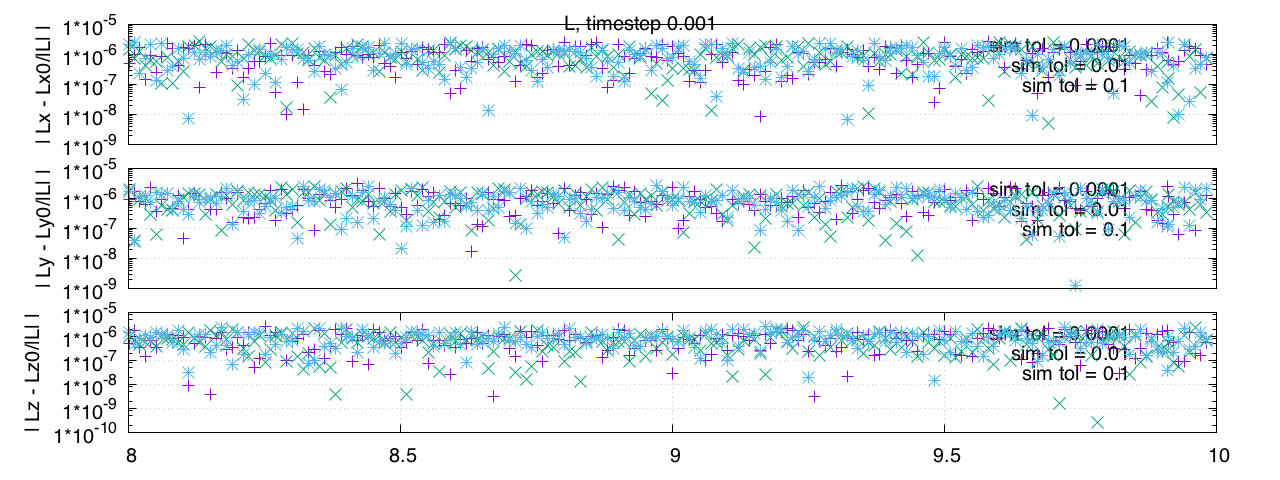
\includegraphics[width=\textwidth]
			{dt_0p001_Lxyz_vs_sampleTime_endtime_0p001.png}}
		\caption{timestep $1 \times 10^{-4}$, $\frac{t}{T}$ from $8$ to $10$}
	\end{subfigure}
	\hfill
	% 98-100 t/T
	\begin{subfigure}[b]{0.49\textwidth}
		{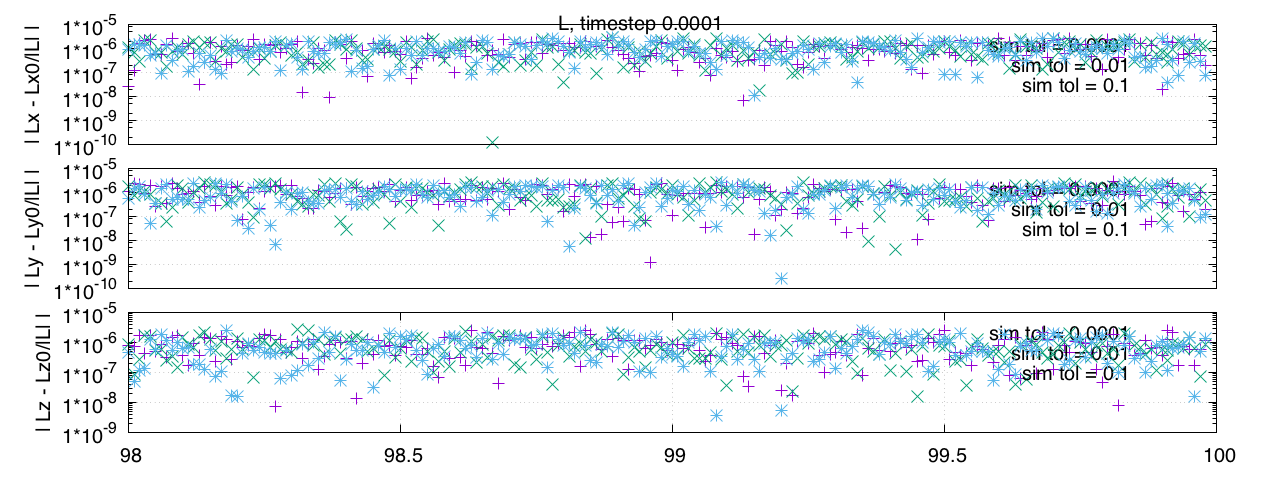
\includegraphics[width=\textwidth]
			{dt_0p0001_Lxyz_vs_sampleTime_endtime_0p01.png}}
		\caption{timestep $1 \times 10^{-4}$, $\frac{t}{T}$ from $98$ to $100$}
	\end{subfigure}
	\vfill
	% TOLERANCE 1 * 10^{-5}
	% 8-10 t/T
	\begin{subfigure}[b]{0.49\textwidth}
		{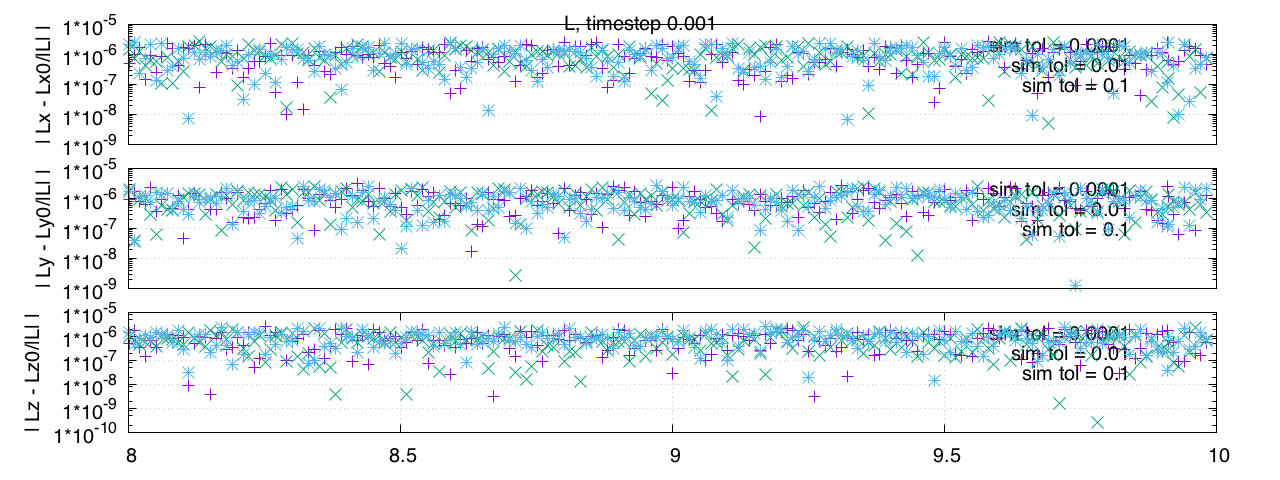
\includegraphics[width=\textwidth]
			{dt_0p001_Lxyz_vs_sampleTime_endtime_0p001.png}}
		\caption{timestep $1 \times 10^{-3}$, $\frac{t}{T}$ from $8$ to $10$}
	\end{subfigure}
	\hfill
	% 98-100 t/T
	\begin{subfigure}[b]{0.49\textwidth}
		{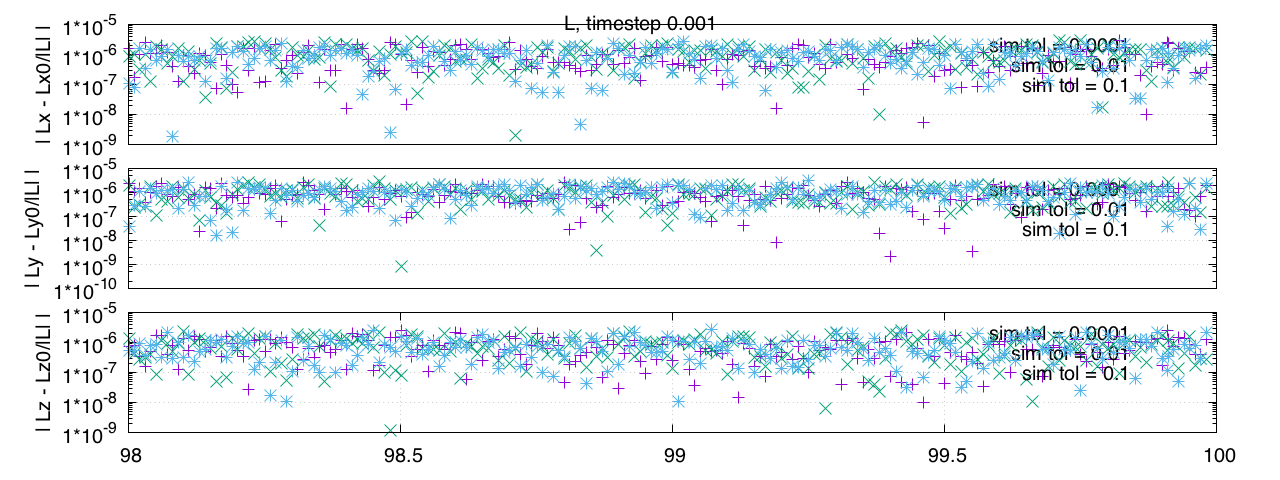
\includegraphics[width=\textwidth]
			{dt_0p001_Lxyz_vs_sampleTime_endtime_0p01.png}}
		\caption{timestep $1 \times 10^{-3}$, $\frac{t}{T}$ from $98$ to $100$}
	\end{subfigure}
	\vfill
	% TOLERANCE 1 * 10^{-3}
	% 8-10 t/T
	\begin{subfigure}[b]{0.49\textwidth}
		{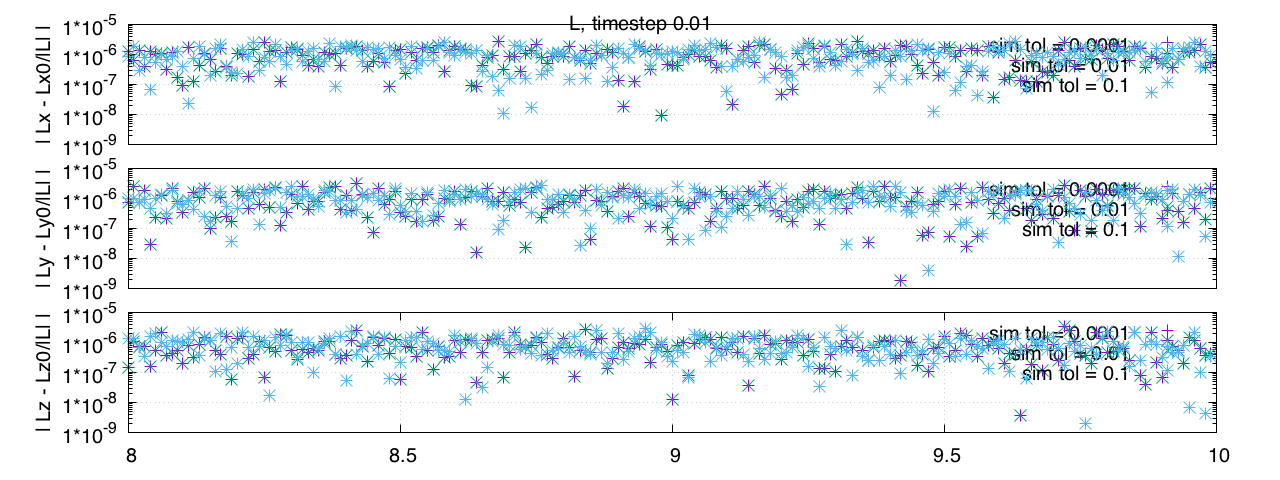
\includegraphics[width=\textwidth]
			{dt_0p01_Lxyz_vs_sampleTime_endtime_0p001.png}}
		\caption{timestep $1 \times 10^{-2}$, $\frac{t}{T}$ from $8$ to $10$}
	\end{subfigure}
	\hfill
	% 98-100 t/T
	\begin{subfigure}[b]{0.49\textwidth}
		{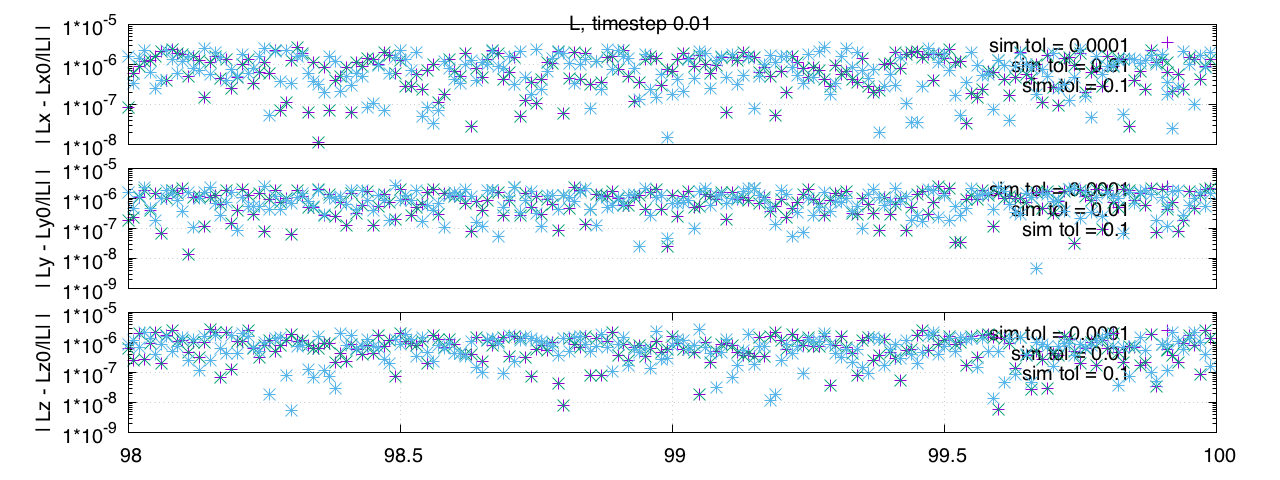
\includegraphics[width=\textwidth]
			{dt_0p01_Lxyz_vs_sampleTime_endtime_0p01.png}}
		\caption{timestep $1 \times 10^{-2}$, $\frac{t}{T}$ from $98$ to $100$}
	\end{subfigure}
	\vfill
	% TOLERANCE 1 * 10^{-1}
	% 8-10 t/T
	\begin{subfigure}[b]{0.49\textwidth}
		{\includegraphics[width=\textwidth]
			{dt_0p1_Lxyz_vs_sampleTime_endtime_0p001.png}}
		\caption{timestep $1 \times 10^{-1}$, $\frac{t}{T}$ from $8$ to $10$}
	\end{subfigure}
	\hfill
	% 98-100 t/T
	\begin{subfigure}[b]{0.49\textwidth}
		{\includegraphics[width=\textwidth]
			{dt_0p1_Lxyz_vs_sampleTime_endtime_0p01.png}}
		\caption{timestep $1 \times 10^{-1}$, $\frac{t}{T}$ from $98$ to $100$}
	\end{subfigure}
	\caption{\label{fig:res-lxyz-1} Component-wise angular momentum of the molecule, at various timesteps levels and  different times ($\frac{t}{T} \in \left[ 8, 10\right] \cup \left[ 98, 100\right]$) during the simulation. The two different tolerances in the $\textsf{RATTLE}$ algorithm were set equal.}
\end{figure}
%%%%%%%%%%%%%%%%%%%%%%%%%%%%%%%%%%%%%%%%%%%%%%%%%%%%